
%(BEGIN_QUESTION)
% Copyright 2006, Tony R. Kuphaldt, released under the Creative Commons Attribution License (v 1.0)
% This means you may do almost anything with this work of mine, so long as you give me proper credit

Følgende lagertank inneholder vann.  En pneumatisk trykktransmitter i bunnen av tanken beregner væskenivå fra hydrostatisk trykk (head).  Bestem kalibreringsområdet for transmitteren slik at tanknivåområdet (0 til 18 fot) oversettes korrekt til et utgangssignal på 3 til 15 PSI.  Oppgi transmitterens kalibreringsområde i tommer W.C. (inches of water column).

$$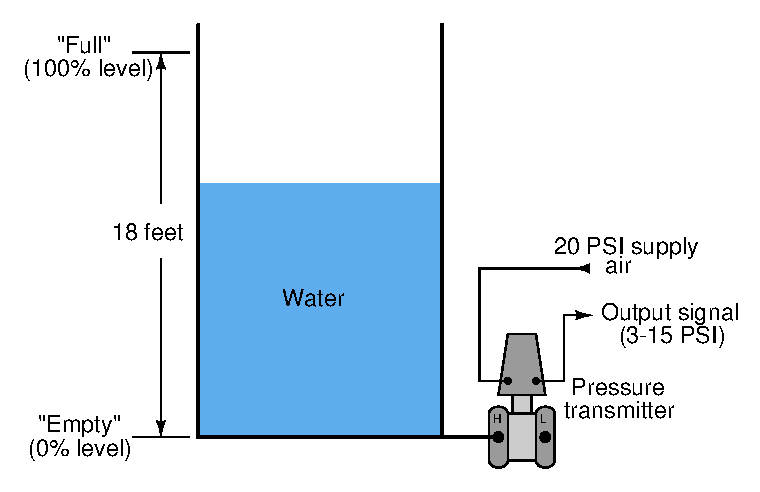
\includegraphics[width=15.5cm]{i00243x01.eps}$$

Bestem deretter følgende (forutsatt at transmitteren er korrekt kalibrert for applikasjonen):

\begin{itemize}
\item{} Transmitterens utgangssignal (PSI) ved 12 fot nivå
\item{} Vannivå ved 5.9 PSI utgangssignal
\end{itemize}

\underbar{file i00243}
%(END_QUESTION)





%(BEGIN_ANSWER)

Nedre måleverdi (LRV): 0 inches W.C. innsignal = 3 PSI utsignal

\vskip 10pt

Øvre måleverdi (URV): 216 inches W.C. innsignal = 15 PSI utsignal

\vskip 10pt

\begin{itemize}
\item{} Transmitterutgang (PSI) ved 12 fot nivå = 11 PSI
\item{} Vannivå ved 5.9 PSI utsignal = 4.35 fot
\end{itemize}

%(END_ANSWER)





%(BEGIN_NOTES)

%INDEX% Measurement, level: hydrostatic pressure

%(END_NOTES)
